\documentclass[UTF8,a4paper,oneside,zihao=-4]{ctexart}

\usepackage{cnarticle}

\graphicspath{{figures/}}
\newcommand{\TotalTrials}{675}
\newcommand{\TotalSubjects}{5}
\newcommand{\OscTrials}{450}
\newcommand{\RotTrials}{225}
\newcommand{\OscAbsMean}{20.04}
\newcommand{\OscAbsMedian}{14.73}
\newcommand{\OscRelMean}{12.45}
\newcommand{\OscRelMedian}{9.61}
\newcommand{\RotAbsMean}{37.23}
\newcommand{\RotAbsMedian}{29.53}
\newcommand{\RotRelMean}{20.68}
\newcommand{\RotRelMedian}{16.41}
\newcommand{\TimingImputations}{3}
\newcommand{\MaxRtEstimateSec}{189.16}
\newcommand{\OscEnergyAbsRho}{0.20}
\newcommand{\OscEnergyRelRho}{-0.18}
\newcommand{\RotEnergyAbsRho}{0.10}
\newcommand{\RotEnergyRelRho}{0.10}

\newcommand{\GeneratedOverallRows}{%
摆动 & 450 & 20.04 $\pm$ 19.89 & 14.73 [5.64, 29.09] & 12.45 $\pm$ 11.12 & 9.61 [3.32, 18.53] \\
旋转 & 225 & 37.23 $\pm$ 33.19 & 29.53 [14.11, 51.47] & 20.68 $\pm$ 18.44 & 16.41 [7.84, 28.60] \\
}

\newcommand{\GeneratedSubjectRows}{%
E2-0001 & 18.89 & 30.63 & 12.64 & 17.02 & 11.73 \\
E2-0002 & 19.73 & 31.65 & 12.16 & 17.58 & 11.92 \\
E2-0003 & 15.22 & 29.41 & 10.07 & 16.34 & 14.19 \\
E2-0004 & 11.93 & 21.38 & 7.28 & 11.88 & 9.45 \\
E2-0005 & 34.42 & 73.07 & 20.10 & 40.60 & 38.65 \\
}

\newcommand{\GeneratedTimingRows}{%
遮挡时长（s） & 摆动 & 0.80 & 150 & 18.06 & 12.80 & 11.65 \\
遮挡时长（s） & 摆动 & 1.00 & 150 & 20.67 & 16.69 & 12.71 \\
遮挡时长（s） & 摆动 & 1.20 & 150 & 21.38 & 14.69 & 12.99 \\
遮挡时长（s） & 旋转 & 0.80 & 75 & 34.69 & 27.36 & 19.27 \\
遮挡时长（s） & 旋转 & 1.00 & 75 & 37.97 & 33.37 & 21.10 \\
遮挡时长（s） & 旋转 & 1.20 & 75 & 39.02 & 32.01 & 21.68 \\
显示时长（周期） & 摆动 & 1.25 & 150 & 20.65 & 15.13 & 12.98 \\
显示时长（周期） & 摆动 & 1.50 & 150 & 19.47 & 14.66 & 12.03 \\
显示时长（周期） & 摆动 & 1.75 & 150 & 20.00 & 14.37 & 12.35 \\
显示时长（周期） & 旋转 & 2.50 & 75 & 38.36 & 32.73 & 21.31 \\
显示时长（周期） & 旋转 & 3.00 & 75 & 39.41 & 32.01 & 21.89 \\
显示时长（周期） & 旋转 & 3.50 & 75 & 33.92 & 27.36 & 18.85 \\
}

\newcommand{\GeneratedEnergyRows}{%
摆动 & 5.43 & 45 & 10.40 & 9.79 & 17.03 & 16.03 \\
摆动 & 12.38 & 45 & 12.16 & 10.12 & 12.98 & 10.80 \\
摆动 & 19.33 & 45 & 15.39 & 12.27 & 12.92 & 10.30 \\
摆动 & 26.28 & 45 & 22.53 & 20.32 & 15.92 & 14.36 \\
摆动 & 33.23 & 45 & 19.85 & 16.69 & 12.22 & 10.27 \\
摆动 & 40.18 & 45 & 22.21 & 14.07 & 12.15 & 7.69 \\
摆动 & 47.13 & 45 & 21.02 & 17.17 & 10.34 & 8.44 \\
摆动 & 54.08 & 45 & 25.58 & 18.25 & 11.39 & 8.13 \\
摆动 & 61.03 & 45 & 22.49 & 10.07 & 9.08 & 4.07 \\
摆动 & 67.98 & 45 & 28.76 & 22.64 & 10.48 & 8.25 \\
旋转 & 85.75 & 45 & 33.85 & 25.36 & 18.81 & 14.09 \\
旋转 & 90.65 & 45 & 39.33 & 32.01 & 21.85 & 17.78 \\
旋转 & 95.55 & 45 & 33.02 & 21.25 & 18.35 & 11.81 \\
旋转 & 100.45 & 45 & 34.40 & 31.52 & 19.11 & 17.51 \\
旋转 & 105.35 & 45 & 45.54 & 34.86 & 25.30 & 19.36 \\
}


\title{实验二颜色速度提示条件下的终态位置估计误差分析}
\shorttitle{实验二终态位置估计误差分析}
\author{}
\date{2026年9月30日}

\begin{document}

\maketitle

\begin{abstract}
本报告对实验二5名被试的\TotalTrials{}个正式试次进行描述性分析。每名被试均完成90个摆动试次和45个旋转试次。绝对误差采用被试估计角与真实终态角之间的有效角距离；相对误差以该试次的最大可能角误差为分母，从而避免真实角度接近零时比值失稳。摆动条件的平均绝对误差为\OscAbsMean{}°，平均相对误差为\OscRelMean{}\%；旋转条件分别为\RotAbsMean{}°和\RotRelMean{}\%。五名被试的旋转误差均高于摆动误差，但被试间差异明显。遮挡时长只呈现轻微且不完全一致的趋势，显示时长与误差之间没有清晰的单调关系。鉴于被试数量较少，本文仅报告描述统计，不进行群体显著性推断。
\end{abstract}

\keywords{直觉物理；单摆；终态估计；绝对误差；相对误差；相空间}

\section{数据与方法}
\label{sec:method}

\subsection{数据范围}

分析使用5个状态为完成的实验二CSV文件，只纳入正式阶段数据，不包含练习试次。数据共\TotalTrials{}行，来自\TotalSubjects{}名匿名被试；其中摆动条件\OscTrials{}个试次，旋转条件\RotTrials{}个试次。每名被试均有135个正式试次，分别包含90个摆动试次和45个旋转试次，因此不同被试在同一运动条件下具有相同权重。

实验中的摆动条件包含10个能量水平，旋转条件包含5个能量水平，每个能量水平在合并数据中均有45个试次。遮挡时长为0.8、1.0或1.2秒；摆动的显示时长为1.25、1.50或1.75个周期，旋转的显示时长为2.50、3.00或3.50个周期。

\subsection{误差定义}

设真实终态角为$\theta_i$，被试估计角为$\hat{\theta}_i$。绝对角误差记为$e_i$。对于旋转试次，$e_i$为圆周上的最短角距离；对于摆动试次，先将估计角限制在该试次允许的$[-w_{\max,i},w_{\max,i}]$范围内，再计算其与真实角的距离。角度均以度为单位。

为了使摆动和旋转条件能够在不同响应范围下比较，本报告将相对误差定义为绝对误差占该试次最大可能角误差的百分比：
\begin{equation}
    r_i=100\%\times\frac{e_i}{e_{\max,i}},\qquad
    e_{\max,i}=\begin{cases}
        2w_{\max,i}, & \text{摆动},\\
        180^\circ, & \text{旋转}.
    \end{cases}
    \label{eq:relative-error}
\end{equation}
这一指标的理论范围为0\%至100\%。它不同于$e_i/|\theta_i|$：后者会因角度零点的选择以及真实角接近0°而产生极端比值，不适合本数据的相空间任务。

\subsection{统计方法}

报告同时给出均值、标准差、中位数、四分位距和范围。条件比较以描述性结果为主，并分别查看运动类别、被试、遮挡时长、显示时长、能量水平和隐藏阶段是否发生转向。能量与误差的关系使用Spearman等级相关系数作描述，不计算显著性。由于只有5名被试，试次级观测也不是相互独立的，本报告不进行假设检验或群体效应推断。

\section{数据质量}
\label{sec:quality}

5个数据文件均通过完整性检查。每名被试的正式响应序号唯一覆盖1至135；未发现重复的试次标识或“被试--正式序号”组合，终态角、估计角、误差和反应时等核心字段没有缺失。根据原始角度重新计算绝对误差后，与导出字段的最大差异为$6.93\times10^{-14}$°，可视为浮点舍入误差。

原始记录中有\TimingImputations{}个试次受到页面隐藏计时程序错误影响。预处理时，将每个异常试次与其余被试中能量、显示时长和遮挡时长完全相同的4个正常试次匹配，并以对应反应时的中位数填补；三个修正值分别为4.34、2.21和3.41秒，同时将页面隐藏次数与时长归零。仿真轨迹、终态、估计角和误差字段均未修改。修正后最长反应时为\MaxRtEstimateSec{}秒；反应时仍不作为本报告的主要结果。最大单帧间隔为96.8毫秒，未发现由此造成的缺失响应。

\section{结果}
\label{sec:results}

\subsection{运动条件的总体误差}

\begin{table}[htbp]
    \centering
    \caption{两类运动条件的误差汇总}
    \label{tab:overall-errors}
    \small
    \setlength{\tabcolsep}{4.5pt}
    \begin{tabularx}{\linewidth}{@{}l r c X c X@{}}
        \toprule
        条件 & $n$ & 绝对误差均值 $\pm$ 标准差（°） & 绝对误差中位数 [Q1, Q3]（°） & 相对误差均值 $\pm$ 标准差（\%） & 相对误差中位数 [Q1, Q3]（\%） \\
        \midrule
        \GeneratedOverallRows
        \bottomrule
    \end{tabularx}
\end{table}

如\cref{tab:overall-errors}所示，旋转条件的平均绝对误差为\RotAbsMean{}°，高于摆动条件的\OscAbsMean{}°；其中位数也从\OscAbsMedian{}°升至\RotAbsMedian{}°。范围归一化后，旋转条件的平均相对误差仍为\RotRelMean{}\%，高于摆动条件的\OscRelMean{}\%。因此，旋转条件的较大绝对误差不能仅由其角度范围更宽解释。

两类条件的均值均高于中位数，且最大绝对误差分别达到140.84°和161.80°，说明分布右偏并含有少量大误差试次。基于这一特征，后续结果同时保留均值和中位数，不用单一均值概括表现。\cref{fig:error-distributions}进一步展示了全部试次的分布形态。

\begin{figure}[htbp]
    \centering
    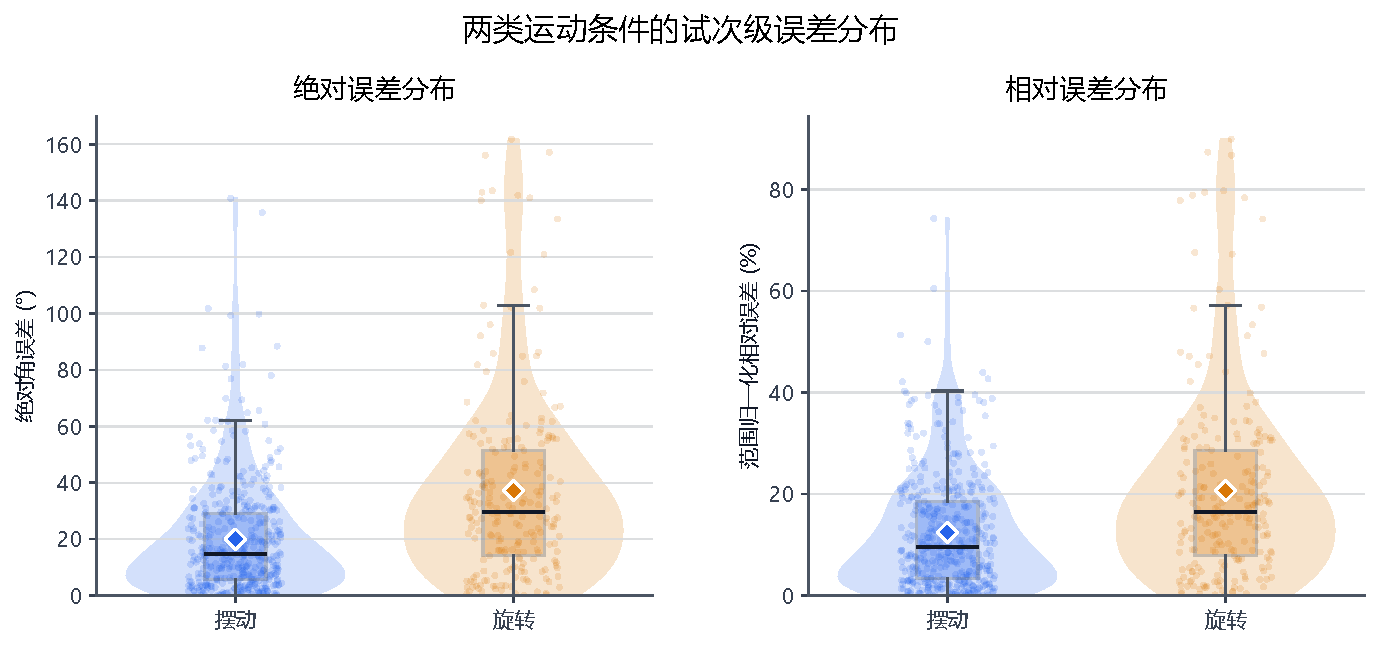
\includegraphics[width=0.96\linewidth]{error-distributions.pdf}
    \caption{摆动和旋转条件下的试次级绝对误差与范围归一化相对误差分布。小提琴轮廓表示分布密度，箱体表示四分位范围和中位数，半透明点表示单个试次，菱形表示均值。}
    \label{fig:error-distributions}
\end{figure}

\subsection{被试间差异}

\begin{figure}[htbp]
    \centering
    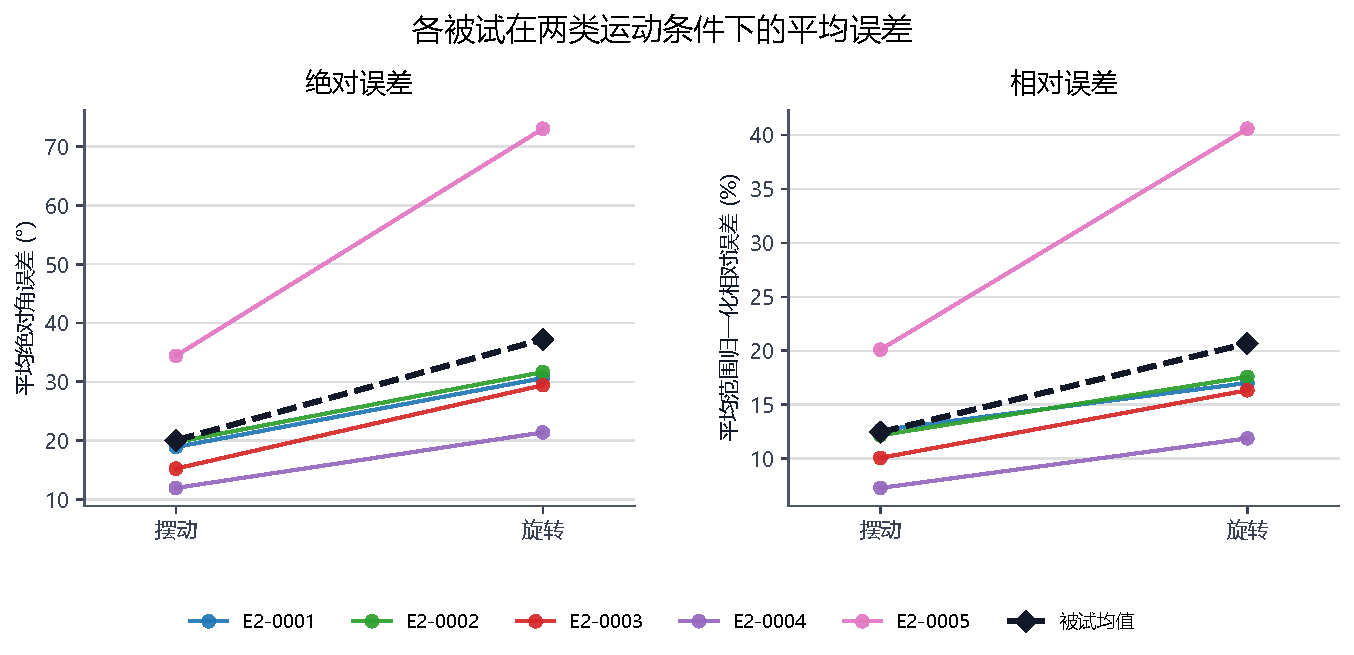
\includegraphics[width=0.96\linewidth]{subject-paired-errors.pdf}
    \caption{各被试在摆动和旋转条件下的平均绝对误差与范围归一化相对误差。彩色线表示单名被试，黑色虚线表示五名被试均值。}
    \label{fig:subject-pairs}
\end{figure}

\begin{table}[htbp]
    \centering
    \caption{各被试的平均误差}
    \label{tab:subject-errors}
    \footnotesize
    \setlength{\tabcolsep}{3.2pt}
    \begin{tabularx}{\linewidth}{@{}l *{5}{>{\centering\arraybackslash}X}@{}}
        \toprule
        被试 & \shortstack{摆动绝对\\误差（°）} & \shortstack{旋转绝对\\误差（°）} & \shortstack{摆动相对\\误差（\%）} & \shortstack{旋转相对\\误差（\%）} & \shortstack{绝对误差\\差值（°）} \\
        \midrule
        \GeneratedSubjectRows
        \bottomrule
    \end{tabularx}
\end{table}

\cref{fig:subject-pairs}和\cref{tab:subject-errors}显示，五名被试的旋转平均误差均高于其摆动平均误差，绝对误差差值介于9.45°和38.65°之间。E2-0005在两类条件下的误差均最高，且旋转条件增幅最大；E2-0004在两类条件下的误差最低。该差异表明个体表现对合并均值有明显影响，尤其不能把所有试次直接视为来自同一个同质总体。

\subsection{终态相空间中的误差分布}

\begin{figure}[htbp]
    \centering
    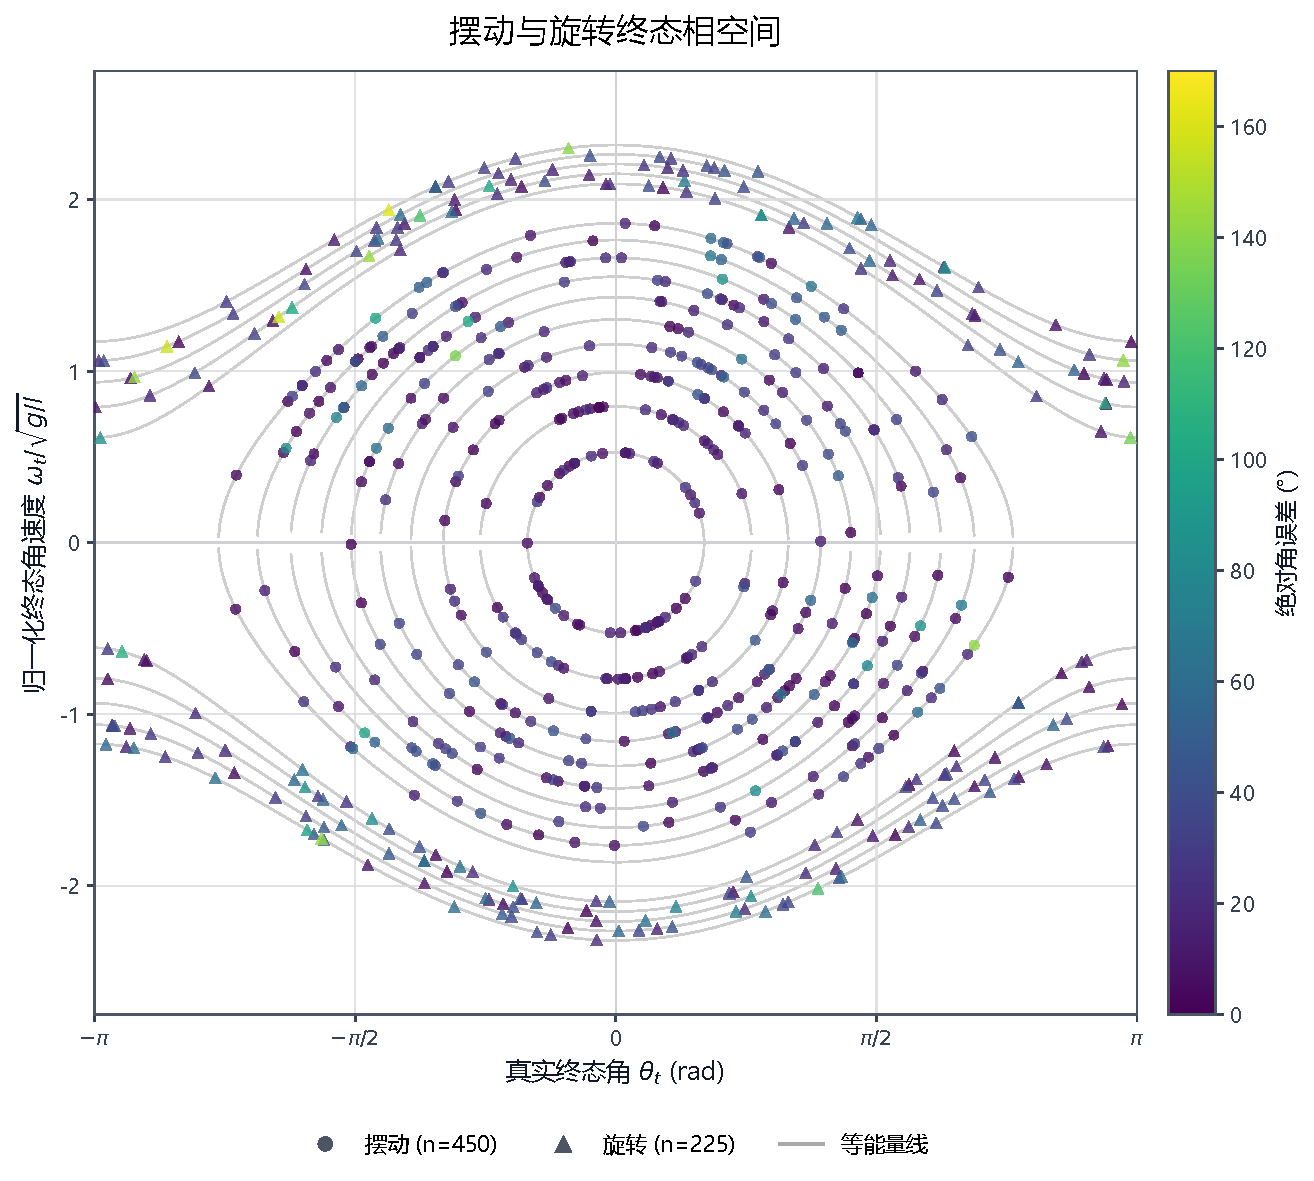
\includegraphics[width=0.98\linewidth]{phase-space-error.pdf}
    \caption{真实终态在同一相空间中的分布。圆点表示摆动试次，三角形表示旋转试次；点颜色表示被试估计与真实终态之间的绝对角误差。角速度用单摆自然频率$\sqrt{g/l}$归一化，浅灰线为15个实验能量水平对应的等能量轨迹。}
    \label{fig:phase-space}
\end{figure}

\cref{fig:phase-space}中的观测点沿设计能量轨迹分布，摆动试次形成闭合轨道，旋转试次位于临界能量之外。大误差点没有集中在单一终态角或单一角速度区域，但在旋转轨迹及部分高能量摆动轨迹上更常见。该图主要用于定位误差在状态空间中的位置，不将点的局部聚集解释为独立统计证据。

\subsection{时序、能量与隐藏阶段转向}

\begin{table}[htbp]
    \centering
    \caption{遮挡和显示时长下的误差汇总}
    \label{tab:timing-errors}
    \footnotesize
    \setlength{\tabcolsep}{4.2pt}
    \begin{tabularx}{\linewidth}{@{}l l r r r r r@{}}
        \toprule
        因素 & 条件 & 水平 & $n$ & 绝对误差均值（°） & 绝对误差中位数（°） & 相对误差均值（\%） \\
        \midrule
        \GeneratedTimingRows
        \bottomrule
    \end{tabularx}
\end{table}

\begin{figure}[htbp]
    \centering
    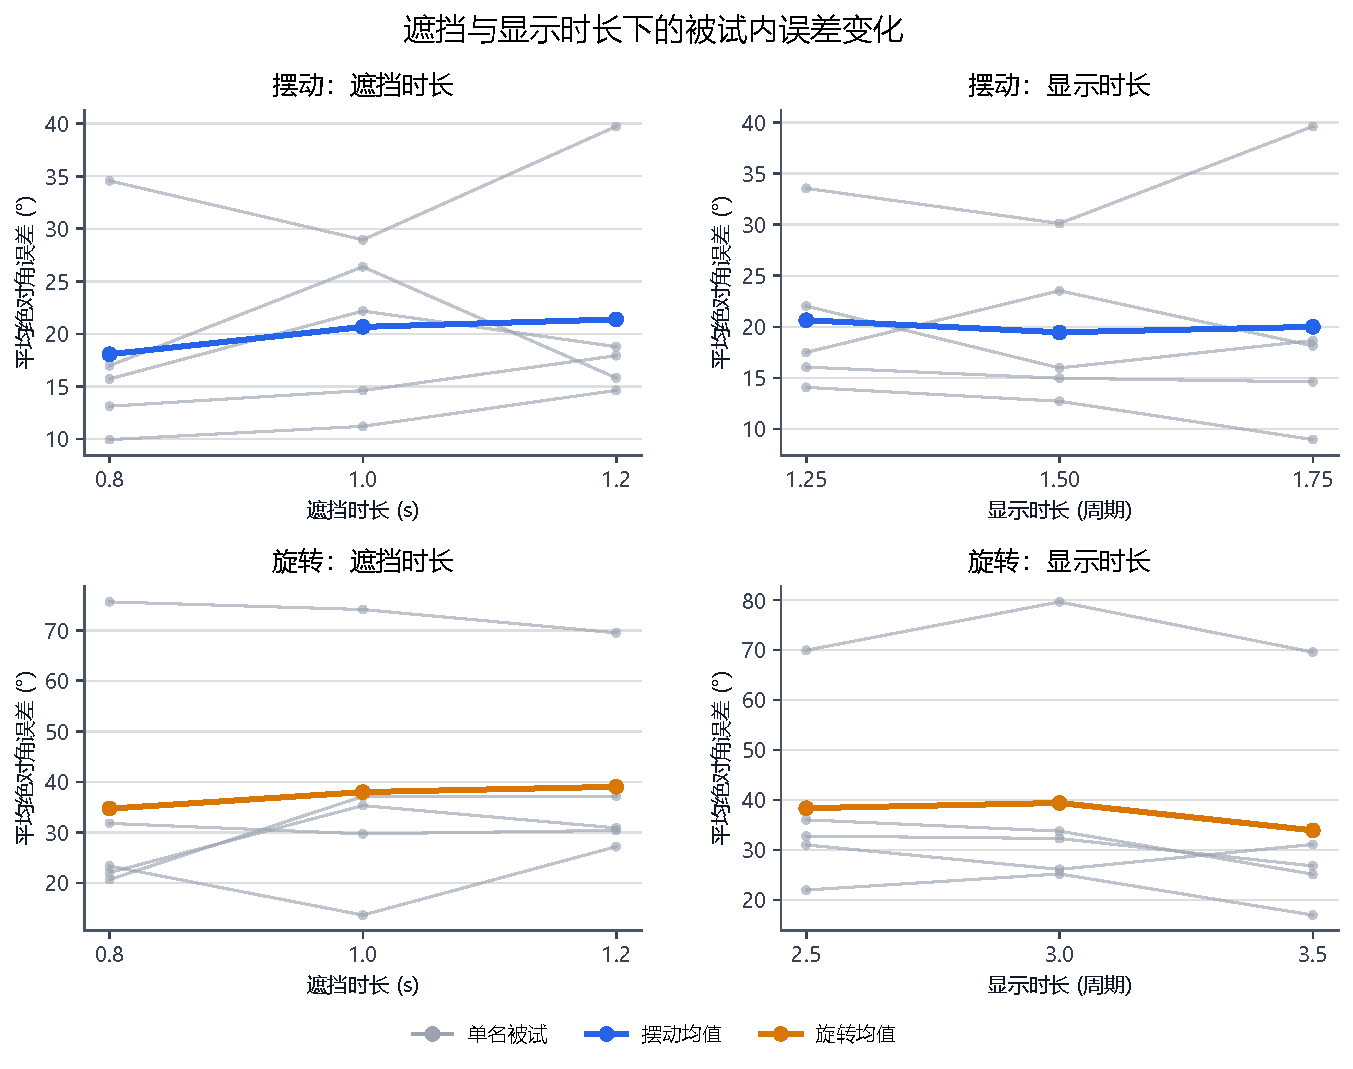
\includegraphics[width=0.96\linewidth]{timing-effects.pdf}
    \caption{遮挡时长和显示时长下的被试内平均绝对误差。灰线表示单名被试，彩色粗线表示五名被试均值。不同被试的变化方向并不完全一致。}
    \label{fig:timing-effects}
\end{figure}

合并所有被试后，遮挡时间从0.8秒增加到1.2秒时，摆动条件的平均绝对误差由18.06°增至21.38°，旋转条件由34.69°增至39.02°；相对误差均值分别增加1.34和2.41个百分点。\cref{fig:timing-effects}显示这个变化较小，而且各被试的变化方向并不完全一致，因此只能视为描述性趋势。

显示时长没有清晰的单调关系。摆动条件三个显示水平的平均绝对误差介于19.47°至20.65°；旋转条件在2.5、3.0和3.5个周期下分别为38.36°、39.41°和33.92°。现有样本不足以判断较长显示是否稳定改善表现。

能量水平与绝对误差的等级相关较弱：摆动和旋转条件分别为$\rho=\OscEnergyAbsRho{}$和$\rho=\RotEnergyAbsRho{}$。摆动条件的相对误差与能量呈轻微负相关（$\rho=\OscEnergyRelRho{}$），主要因为高能量试次的允许角度范围更大；旋转条件的相对误差相关为$\rho=\RotEnergyRelRho{}$。\cref{fig:energy-effects}给出各能量水平的五名被试均值及被试间范围，完整数值见\cref{tab:energy-errors}。

\begin{figure}[htbp]
    \centering
    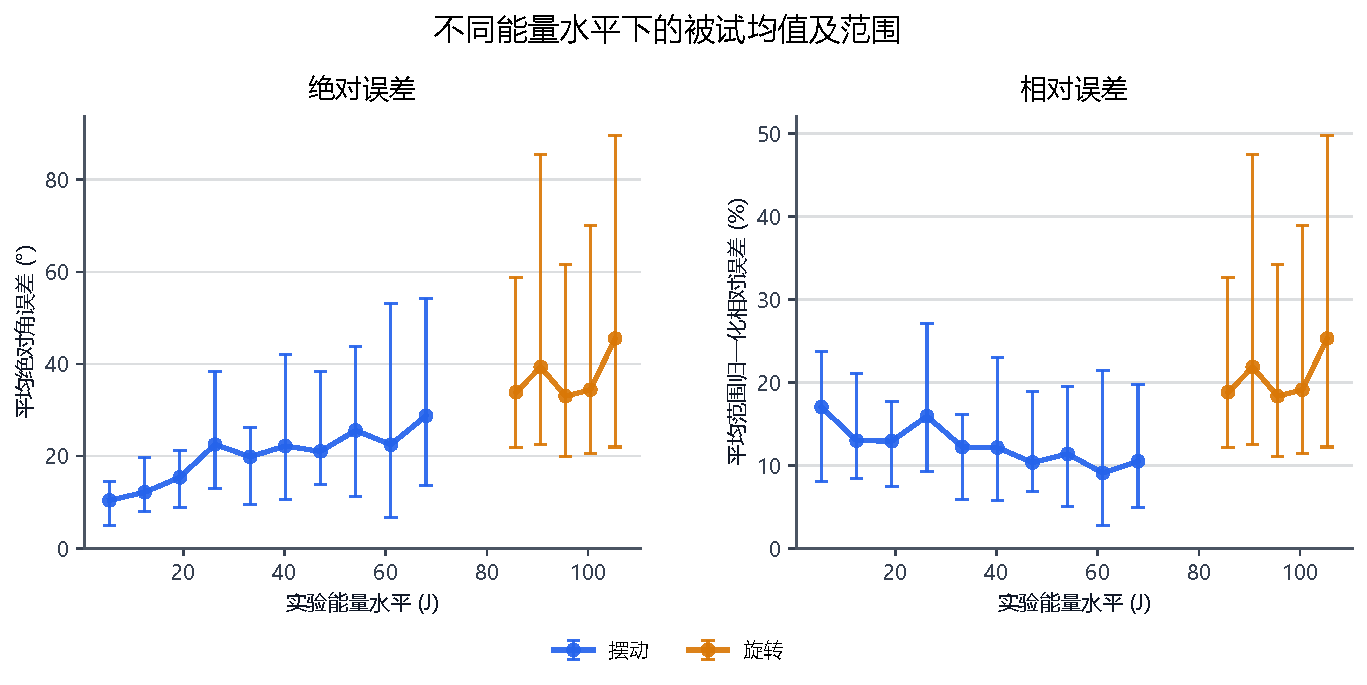
\includegraphics[width=0.96\linewidth]{energy-effects.pdf}
    \caption{不同实验能量水平下的误差。点为五名被试均值，误差线表示五名被试均值的最小值至最大值范围；该范围用于呈现个体差异，不表示置信区间。}
    \label{fig:energy-effects}
\end{figure}

在摆动试次中，隐藏阶段未发生转向与发生转向各有225个试次。两组平均绝对误差分别为22.01°和18.07°，中位数分别为19.13°和10.12°。虽然合并结果中发生转向的试次误差较低，但考虑到明显的个体差异，本报告不将其解释为转向带来优势。

\section{讨论}
\label{sec:discussion}

本数据最稳定的描述性结果是旋转条件比摆动条件产生更大的终态位置估计误差。该差异在五名被试中方向一致，并且在按最大可能角误差归一化后仍然存在，说明结果不只是两类运动角度范围不同造成的。旋转运动需要在遮挡期间持续追踪绕轴运动并处理角度周期性，这可能增加内部模拟难度；不过本报告没有操纵或测量具体认知机制，因此不能据此确定原因。

第二个明显特征是个体差异。E2-0005的平均误差显著高于其他被试，并明显抬高旋转条件的合并均值。中位数与被试内配对结果仍支持旋转误差较大，但未来扩大样本后应使用以被试为分析单位的模型，并考虑稳健统计或分层模型，而不应仅依赖试次级均值。

遮挡时长呈现轻微的误差增加，显示时长、能量水平和隐藏阶段转向则没有一致而简单的模式。这些因素可能与运动类别、能量和被试策略共同作用。现阶段更适合把这些结果作为后续建模线索，而不是得出确定效应结论。

\section{局限}
\label{sec:limitations}

本报告仅包含5名被试，无法可靠估计群体差异，也不适合进行常规显著性检验。每名被试贡献多个重复试次，试次之间不应视为完全独立。分析尚未显式控制试次顺序、Block顺序、练习或疲劳效应，也未建立被试层面的随机效应模型。相对误差采用最大可能角误差归一化，便于跨运动类别比较，但其含义是“占最大可能错误的比例”，不是传统的“相对于真实角度大小”的比值。

\section{结论}
\label{sec:conclusion}

实验二当前数据完整，误差字段可由原始角度准确复算。五名被试在旋转条件下均表现出比摆动条件更大的绝对误差和范围归一化相对误差。被试间差异较大，而遮挡时长、显示时长、能量和隐藏转向的模式较弱或不一致。现有结果支持把运动类别和个体差异作为后续分析重点，但在扩大被试样本并采用被试层级模型之前，不宜作群体因果推断。

\appendix
\section{各能量水平的描述统计}
\label{sec:energy-appendix}

{\footnotesize
\setlength{\tabcolsep}{3pt}
\begin{longtable}{@{}llrrrrr@{}}
    \caption{各能量水平的误差汇总}\label{tab:energy-errors}\\
    \toprule
    条件 & \shortstack{能量\\（J）} & $n$ & \shortstack{绝对误差\\均值（°）} & \shortstack{绝对误差\\中位数（°）} & \shortstack{相对误差\\均值（\%）} & \shortstack{相对误差\\中位数（\%）} \\
    \midrule
    \endfirsthead
    \multicolumn{7}{c}{\tablename\ \thetable\ （续）}\\
    \toprule
    条件 & \shortstack{能量\\（J）} & $n$ & \shortstack{绝对误差\\均值（°）} & \shortstack{绝对误差\\中位数（°）} & \shortstack{相对误差\\均值（\%）} & \shortstack{相对误差\\中位数（\%）} \\
    \midrule
    \endhead
    \midrule
    \multicolumn{7}{r}{续下页}\\
    \endfoot
    \bottomrule
    \endlastfoot
    \GeneratedEnergyRows
\end{longtable}
}

\end{document}
